\documentclass{ieeetran}

\usepackage[utf8]{inputenc}                 % allow utf-8 text in the source
\usepackage[T1]{fontenc}                    % allow proper hyphenation/copy-paste (http://tex.stackexchange.com/a/677) 
\usepackage{blindtext}                      % for generating sample text
\usepackage{amsmath}
\usepackage[inline]{enumitem}               % inline enumeration support
\usepackage[pdftex]{xcolor,graphicx}        % improved colors and graphics
\usepackage[font=footnotesize]{subcaption}  % subcaptions
\usepackage{xspace}
\usepackage{soul}                           % text highlighting
\usepackage[pdftex]{hyperref}               % pdflatex goodies

% hyperref setup (http://www.andy-roberts.net/misc/latex/pdftutorial.html)
\hypersetup{
    pdfstartview=FitH,
    pdftitle={...},
    pdfauthor={Manolis Stamatogiannakis, Paul Groth, Herbert Bos},
    pdfkeywords={...},
    bookmarks,
    bookmarksopen,
    colorlinks,
    linkcolor=blue,
    citecolor=blue,
    urlcolor=blue,
}

% custom commands
\newcommand{\code}[1]{{\footnotesize\texttt{#1}}}
\newcommand{\figref}[1]{\figurename~\ref{#1}\xspace}
\newcommand{\hlc}[2][yellow]{ {\sethlcolor{#1} \hl{#2}} }

% shorthands
\def\oursystem{\textsf{...}\xspace}

%********************************************************************
%********************************************************************
\begin{document}

%--------------------------------------------------------------------

\title{Just 'cos You Got the Power}
\author{Manolis Stamatogiannakis \and Paul Groth \and Herbert Bos}
\institute{
VU University Amsterdam, The Netherlands,\\
\email{\{manolis.stamatogiannakis, p.t.groth, h.j.bos\}@vu.nl}
}

% lncs overrides
%\titlerunning{Just 'cos You Got the Power}                         % abbreviated title (for running head)
%\authorrunning{Manolis Stamatogiannakis et al.}    % abbreviated author list (for running head)
%\tocauthor{Manolis Stamatogiannakis, Paul Groth, Herbert Bos}
\maketitle

%--------------------------------------------------------------------

\begin{abstract}
\blindtext
\end{abstract}

\begin{keywords}\hlc{kw1, kw2, kw3}\end{keywords}

%--------------------------------------------------------------------

\section{Introduction}
\blindtext[1]
\blindlist{enumerate}[5]
\blindtext[1]
And now an inline enumeration:
\begin{enumerate*}[label=\itshape\alph*\upshape)]
\item Ian ``Lemmy'' Kilmister
\item Phil ``Wizzö'' Campbell
\item Mikkey Dee
\end{enumerate*}.

%--------------------------------------------------------------------

\section{Related work}

See some cool pics in \figref{fig:lucy1} and \figref{fig:lucy2}.
After that, read \cite{Stamatogiannakis:BlackBox:IPAW:2014}.

\begin{figure}[t]
    \centering
    \begin{subfigure}[c]{.45\textwidth}
        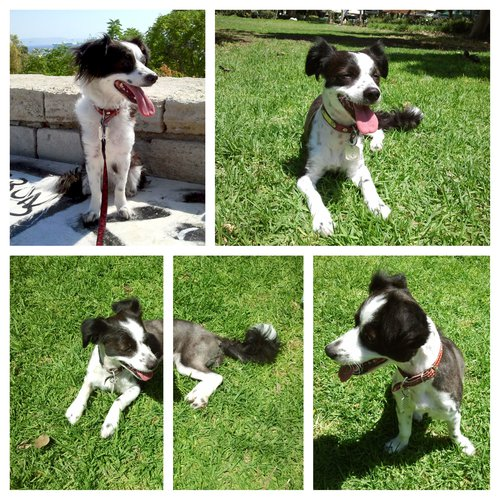
\includegraphics[width=\textwidth]{figs/lucy1}
        % \phantomcaption
        \caption[A cool dog.]{A cool dog.}
        \label{fig:lucy1}
    \end{subfigure}
    \hfill
    \begin{subfigure}[c]{.45\textwidth}
        \centering
        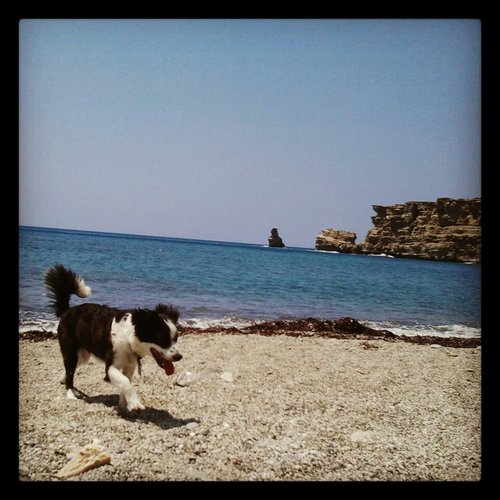
\includegraphics[width=\textwidth]{figs/lucy2}
        % \phantomcaption
        \caption[A cool dog at sea.]{A cool dog at sea.}
        \label{fig:lucy2}
   \end{subfigure}
    \caption[Dog Pictures]{
        Pictures of a cool dog at the park and at sea.
    }
    \label{fig:dogs}
\end{figure}

%--------------------------------------------------------------------

\section{Evaluation}
\blindtext[2]
\blindlist{itemize}[5]
\blindtext[1]

%--------------------------------------------------------------------

\bibliographystyle{splncs03}
\bibliography{references}

%--------------------------------------------------------------------
\end{document}
%********************************************************************
%********************************************************************
